\chapter{Arhitektura i dizajn sustava}

Arhitektura sustava može se podijeliti na tri ključna podsustava:

\begin{packed_enum}
	\item Web poslužitelj:
	\begin{packed_enum}
		\item Srce web aplikacije.
		\item Odgovoran za interakciju između klijenta i aplikacije.
		\item Koristi HTTP/HTTPS protokol za prijenos informacija na webu.
		\item Inicira pokretanje web aplikacije i proslijeđuje zahtjeve.
	\end{packed_enum}
	\item Web aplikacija:
	\begin{packed_enum}
		\item Procesira korisničke zahtjeve i obrađuje ih.
		\item Pristupa bazi podataka prema potrebi.
		\item Generira odgovore u obliku HTML dokumenata za prikaz u web pregledniku.
	\end{packed_enum}			
	\item Baza podataka:	
	\begin{packed_enum}
		\item Sprema podatke koji se koriste ili modificiraju unutar web aplikacije.
	\end{packed_enum}
\end{packed_enum}

Korisnik, putem web preglednika, šalje zahtjeve web poslužitelju. 
Web poslužitelj zatim inicira rad web aplikacije, koja procesira zahtjeve, pristupa bazi podataka po potrebi i vraća odgovore u obliku HTML dokumenata. 
Ova interakcija omogućuje korisnicima pregled i manipulaciju sadržajem putem web sučelja.

\begin{figure}[H]
	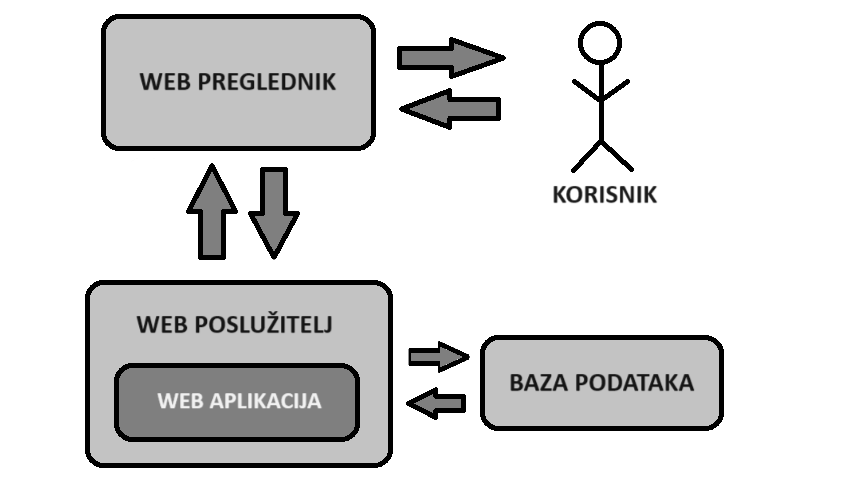
\includegraphics[scale=0.5]{slike/arhitektura.png}
	\centering
	\caption{Arhitektura sustava}
	\label{fig:arhitektura}
\end{figure}

React je biblioteka koju smo odabrali za izradu naše web aplikacije, zajedno sa Spring Boot radnim okvirom te programskim jezikom JavaScript. 
Odabrano razvojno okruženje je Visual Studio Code. Arhitektura sustava temeljiti će se na MVC(Model-View-Controller) konceptu.
\newline React je biblioteka otvorenog koda koja se koristi za izgradnju korisničkih sučelja.
\begin{packed_item}
	\item Jezik: Povezan je s JavaScriptom
	\item Slučajevi upotrebe: Često se koristi za izradu jednostranih aplikacija, gdje je potrebna brza i prilagodljiva interakcija
	\item Platforma: Nema specifičnu platformu; može se koristiti u web aplikacijama na različitim platformama
\end{packed_item}
Spring Boot je radno okruženje koje se koristi za izgradnju aplikacija.
\begin{packed_item}
	\item Jezik: prvenstveno povezan s Javom
	\item Radno okruženje: Spring Boot dio je Spring Frameworka za Java razvoj
	\item Slučajevi upotrebe: naširoko se koristi za izradu web aplikacija temeljenih na Javi
	\item Ekosustav: Java ekosustav, s jakom integracijom s tehnologijama kao što su Spring MVC, Spring Data itd.
	\item Platforma: Java Virtual Machine (JVM)
\end{packed_item}
Spring Boot podržava koncept MVC (Model-View-Controller) arhitekture, a to se postiže kroz Spring Web MVC modul. Spring Boot podržava MVC koncept:
\begin{packed_item}
	\item Model: Spring Boot omogućava korištenje Java objekata kao modela. Ovi objekti predstavljaju podatke koji se koriste u aplikaciji.
	Spring Data može se integrirati za jednostavno upravljanje podacima i komunikaciju s bazom podataka.
	\item View: Spring Boot pruža fleksibilnost u odabiru tehnologije za prikazivanje korisničkog sučelja. Prikazi se često implementiraju kroz HTML datoteke, a moguće je koristiti različite template engines (Thymeleaf, FreeMarker, JSP).
	Pomoću konfiguracija view resolvera jednostavno se integriraju odabrane tehnologije za prikazivanje podataka korisnicima.
	\item Controller: Anotacije poput @Controller i @RestController omogućuju jednostavno označavanje klasa koje djeluju kao kontroleri.
	@RequestMapping i slične anotacije omogućuju mapiranje HTTP zahtjeva na određene metode kontrolera.
	Spring Boot automatski prepoznaje i konfigurira komponente kontrolera.		
\end{packed_item}
Primjena MVC koncepta u Spring Boot-u olakšava održavanje i proširivost aplikacija.
	
				
		\section{Baza podataka}
			    


		Baze podataka neizostavan su dio razvoja programske potpore jer danas gotova svaka domena primjene obiluje mnoštvom podataka koje treba pohraniti na organiziran način kako bi se efikasno dohvaćali, mijenjali i nadopunjavali. Za upravljanje bazom podataka mogu se koristiti različiti sustavi koji obavljaju optimiranje upita i omogućuju rukovanje podatcima. Mi smo odlučili koristiti PostgreSQL koji nam je bio preporučen na kolegiju Baze podataka. \newline Iako stvarni svijet ne možemo prikazati sa svim detaljima, relacijski nam model baze podataka omogućuje vjeran prikaz stvarnosti pomoću relacija u koje pohranjujemo vrijednosti odabranih atributa vezanih uz entitete bitne za domenu primjene. Formalno gledano relacija, tj. instanca relacije, definirana na relacijskoj shemi je skup n-torki, a neformalno možemo reći da je to imenovana dvodimenzionalna tablica. Atributi su imenovani stupci te tablice. ER (Entity-Relationship) model podataka zadržava dobra svojstva relacijskog modela, a uz to omogućuje eksplicitni prikaz semantičkih informacija vezanih uz veze (odnose) između entiteta. Kako bismo prikazali kako su eniteti našeg sustava povezani koristit ćemo ER model baze podataka.
za podataka ove aplikacije sastoji se od sljedećih entiteta:
		\begin{packed_item}
			\item Korisnik
			\item Pozicija tragača
			\item Uloga
			\item Zadatak 
			\item Pripada postaji
			\item Osposobljen za
			\item Akcija
			\item Postaja
			\item Prijevozno sredstvo
			\item Komentar korisnika 
			\item Životinja
			\item Pozicija životinje
		\end{packed_item}


			\subsection{Opis tablica}
			
				
				
				\begin{longtblr}[
					label=none,
					entry=none
					]{
						width = \textwidth,
						colspec={|X[6,l]|X[6, l]|X[20, l]|}, 
						rowhead = 1,
					} %definicija širine tablice, širine stupaca, poravnanje i broja redaka naslova tablice
					\hline \SetCell[c=3]{c}{\textbf{Zadatak}}	 \\ \hline[3pt]
					\SetCell{LightGreen} Šifra Zadatka & INT	&  	Jedinstveni brojčani identifikator zadatka  	\\ \hline
					\SetCell{LightGreen} Korisničko ime & VARCHAR	& 	Korisničko ime korisnika\\ \hline
					Tekst	& VARCHAR & Opis Zadatka  	\\ \hline 
					Završen & BOOLEAN & Status je li zadatak završen  \\ \hline 
          \SetCell{LightBlue} Šifra akcije 	& INT & Jedinstveni brojčani identifikator akcije   	\\ \hline 
          \SetCell{LightBlue} Šifra životinje 	& INT &   Jedinstveni brojčani identifikator životinje  	\\ \hline 
          \SetCell{LightBlue} Šifra vozila 	& INT &  Jedinstveni brojčani identifikator vozila 	\\ \hline 
				\end{longtblr}
				
				\begin{longtblr}[
					label=none,
					entry=none
					]{
						width = \textwidth,
						colspec={|X[6,l]|X[6, l]|X[20, l]|}, 
						rowhead = 1,
					} %definicija širine tablice, širine stupaca, poravnanje i broja redaka naslova tablice
          \hline \SetCell[c=3]{c}{\textbf{Akcija}}	 \\ \hline[3pt]
					\SetCell{LightGreen} Šifra akcije & INT	&  	Jedinstveni ključ za identifikaciju zadatka  	\\ \hline
					Naziv akcije	& VARCHAR &  Puni naziv akcije  	\\ \hline 
					Aktivna & BOOLEAN & Status je li akcija aktvna  \\ \hline 
          \SetCell{LightBlue} Korisničko ime 	& VARCHAR &  Korisničko ime korisnika 	\\ \hline 
				\end{longtblr}
			

				\begin{longtblr}[
					label=none,
					entry=none
					]{
						width = \textwidth,
						colspec={|X[6,l]|X[6, l]|X[20, l]|}, 
						rowhead = 1,
					} %definicija širine tablice, širine stupaca, poravnanje i broja redaka naslova tablice
          \hline \SetCell[c=3]{c}{\textbf{Komentar korisnika}}	 \\ \hline[3pt]
					\SetCell{LightGreen} Šifra životinje & INT	&  	Jedinstveni brojčani identifikator zadatka  	\\ \hline
					\SetCell{LightGreen} Korisničko ime & VARCHAR	&  	Korisničko ime korisnika 	\\ \hline
					\SetCell{LightGreen} Šifra akcije & INT	&  	Jedinstveni brojčani identifikator akcije  	\\ \hline
					Komentar	& VARCHAR & Sadržaj komentara  	\\ \hline 
				\end{longtblr}
			

				\begin{longtblr}[
					label=none,
					entry=none
					]{
						width = \textwidth,
						colspec={|X[6,l]|X[6, l]|X[20, l]|}, 
						rowhead = 1,
					} %definicija širine tablice, širine stupaca, poravnanje i broja redaka naslova tablice
          \hline \SetCell[c=3]{c}{\textbf{Životinja}}	 \\ \hline[3pt]
					\SetCell{LightGreen} Šifra životinje & INT	&  	Jedinstveni brojčani identifikator životinje  	\\ \hline
					Naziv	& VARCHAR & Puni naziv životinje  	\\ \hline 
					Latinski naziv	& VARCHAR & Latinski naziv životinje  	\\ \hline 
					Opis	& VARCHAR & Sadržaj komentara  	\\ \hline 
				\end{longtblr}


				\begin{longtblr}[
					label=none,
					entry=none
					]{
						width = \textwidth,
						colspec={|X[6,l]|X[6, l]|X[20, l]|}, 
						rowhead = 1,
					} %definicija širine tablice, širine stupaca, poravnanje i broja redaka naslova tablice
          \hline \SetCell[c=3]{c}{\textbf{Pozicija životinje}}	 \\ \hline[3pt]
					\SetCell{LightGreen} Šifra životinje & INT	&  	Jedinstveni brojčani identifikator životinje \\ \hline
					\SetCell{LightGreen} Vremenska oznaka & TIMESTAMP	&  	Zadnje vrijeme u kojem je viđena životinja  	\\ \hline
          Geografska širina	& DOUBLE & Iznos geografske širine  	\\ \hline 
          Geografska dužina	& DOUBLE & Iznos geografske dužine  	\\ \hline 
				\end{longtblr}


				\begin{longtblr}[
					label=none,
					entry=none
					]{
						width = \textwidth,
						colspec={|X[6,l]|X[6, l]|X[20, l]|}, 
						rowhead = 1,
					} %definicija širine tablice, širine stupaca, poravnanje i broja redaka naslova tablice
          \hline \SetCell[c=3]{c}{\textbf{Pozicija tragača}}	 \\ \hline[3pt]
					\SetCell{LightGreen} Korisničko ime & VARCHAR	&  	Korisničko ime korisnika  	\\ \hline
					\SetCell{LightGreen} Vremenska oznaka & TIMESTAMP	&  	Zadnje vrijeme kada je tragač zabilježio svoju poziciju  	\\ \hline
					\SetCell{LightGreen} Šifra akcije & INT	&  	Jedinstveni brojčani identifikator akcije  	\\ \hline
          Geografska širina	& DOUBLE & Iznos geografske širine  	\\ \hline 
          Geografska dužina	& DOUBLE & Iznos geografske dužine  	\\ \hline 
				\end{longtblr}


				\begin{longtblr}[
					label=none,
					entry=none
					]{
						width = \textwidth,
						colspec={|X[6,l]|X[6, l]|X[20, l]|}, 
						rowhead = 1,
					} %definicija širine tablice, širine stupaca, poravnanje i broja redaka naslova tablice
          \hline \SetCell[c=3]{c}{\textbf{Korisnik}}	 \\ \hline[3pt]
					\SetCell{LightGreen} Korisničko ime & VARCHAR	&  	Ime korisnika  	\\ \hline
          Email	& VARCHAR & Sadržaj komentara  	\\ \hline 
          Lozinka & VARCHAR & Lozinka korisnika \\ \hline
          Ime & VARCHAR & Ime korisnika \\ \hline
          Prezime & VARCHAR & Prezime korisnika \\ \hline
          Fotografija & VARCHAR & Fotografija korisnika \\ \hline
          \SetCell{LightBlue} Šifra uloge 	& INT &   Jedinstveni brojčani identifikator uloge	\\ \hline 

				\end{longtblr}


				\begin{longtblr}[
					label=none,
					entry=none
					]{
						width = \textwidth,
						colspec={|X[6,l]|X[6, l]|X[20, l]|}, 
						rowhead = 1,
					} %definicija širine tablice, širine stupaca, poravnanje i broja redaka naslova tablice
          \hline \SetCell[c=3]{c}{\textbf{Pripada postaji}}	 \\ \hline[3pt]
					\SetCell{LightGreen} Korisničko ime & VARCHAR	&  	Korisničko ime korisnika  	\\ \hline
					\SetCell{LightGreen} Šifra postaje & VARCHAR	&  	Jedinstveni brojčani identifikator postaje\\ \hline

				\end{longtblr}


				\begin{longtblr}[
					label=none,
					entry=none
					]{
						width = \textwidth,
						colspec={|X[6,l]|X[6, l]|X[20, l]|}, 
						rowhead = 1,
					} %definicija širine tablice, širine stupaca, poravnanje i broja redaka naslova tablice
          \hline \SetCell[c=3]{c}{\textbf{Postaja}}	 \\ \hline[3pt]
					\SetCell{LightGreen} Šifra postaje & VARCHAR	&  	Jedinstveni brojčani identifikator korisnika \\ \hline
					Naziv postaje & VARCHAR	&  	Pun naziv postaje  	\\ \hline

				\end{longtblr}


				\begin{longtblr}[
					label=none,
					entry=none
					]{
						width = \textwidth,
						colspec={|X[6,l]|X[6, l]|X[20, l]|}, 
						rowhead = 1,
					} %definicija širine tablice, širine stupaca, poravnanje i broja redaka naslova tablice
          \hline \SetCell[c=3]{c}{\textbf{Osposobljen za}}	 \\ \hline[3pt]
					\SetCell{LightGreen} Korisničko ime & VARCHAR	&  	Ime korisnika  	\\ \hline
					\SetCell{LightGreen} Šifra vozila & INT	&   Jedinstveni brojčani identifikator vozila  	\\ \hline

				\end{longtblr}


				\begin{longtblr}[
					label=none,
					entry=none
					]{
						width = \textwidth,
						colspec={|X[6,l]|X[6, l]|X[20, l]|}, 
						rowhead = 1,
					} %definicija širine tablice, širine stupaca, poravnanje i broja redaka naslova tablice
          \hline \SetCell[c=3]{c}{\textbf{Prijevozno sredstvo}}	 \\ \hline[3pt]
					\SetCell{LightGreen} Šifra vozila & INT	&   Jedinstveni brojčani identifikator vozila  	\\ \hline
          Naziv vozila & VARCHAR & Puni naziv vozila \\ \hline

				\end{longtblr}


				\begin{longtblr}[
					label=none,
					entry=none
					]{
						width = \textwidth,
						colspec={|X[6,l]|X[6, l]|X[20, l]|}, 
						rowhead = 1,
					} %definicija širine tablice, širine stupaca, poravnanje i broja redaka naslova tablice
          \hline \SetCell[c=3]{c}{\textbf{Uloga}}	 \\ \hline[3pt]
          \SetCell{LightGreen} Šifra Uloge & INT	&  Jedinstveni brojčani identifikator uloge	\\ \hline
          Naziv uloge	& VARCHAR & Puni naziv uloge  	\\ \hline 

				\end{longtblr}


			\subsection{Dijagram baze podataka}

			\begin{figure}[H]
				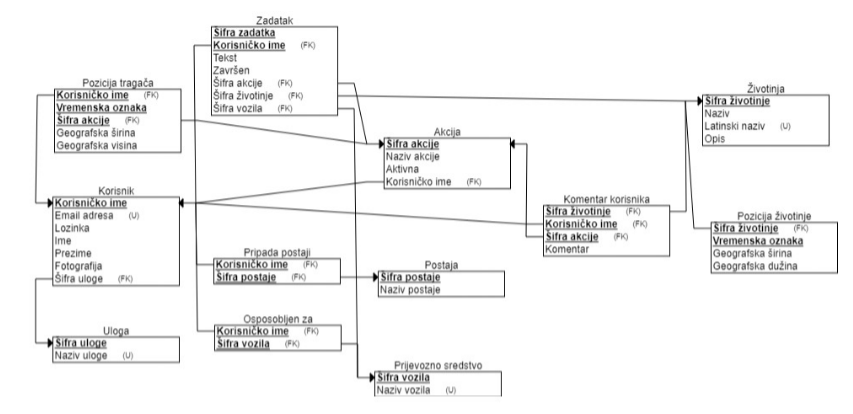
\includegraphics[scale=0.9]{slike/dijagram baze podataka.png} 
				\centering
				\caption{Dijagram baze podataka}
				\label{fig:dijagram_baze_podataka}
			\end{figure}
			
			\eject
			
			
		\section{Dijagram razreda}
		
			\textit{Potrebno je priložiti dijagram razreda s pripadajućim opisom. Zbog preglednosti je moguće dijagram razlomiti na više njih, ali moraju biti grupirani prema sličnim razinama apstrakcije i srodnim funkcionalnostima.}\\
			
			\textbf{\textit{dio 1. revizije}}\\
			
			\textit{Prilikom prve predaje projekta, potrebno je priložiti potpuno razrađen dijagram razreda vezan uz \textbf{generičku funkcionalnost} sustava. Ostale funkcionalnosti trebaju biti idejno razrađene u dijagramu sa sljedećim komponentama: nazivi razreda, nazivi metoda i vrste pristupa metodama (npr. javni, zaštićeni), nazivi atributa razreda, veze i odnosi između razreda.}\\
			
			\textbf{\textit{dio 2. revizije}}\\			
			
			\textit{Prilikom druge predaje projekta dijagram razreda i opisi moraju odgovarati stvarnom stanju implementacije}
			
			
			
			\eject
		
		\section{Dijagram stanja}
			
			
			\textbf{\textit{dio 2. revizije}}\\
			
			\textit{Potrebno je priložiti dijagram stanja i opisati ga. Dovoljan je jedan dijagram stanja koji prikazuje \textbf{značajan dio funkcionalnosti} sustava. Na primjer, stanja korisničkog sučelja i tijek korištenja neke ključne funkcionalnosti jesu značajan dio sustava, a registracija i prijava nisu. }
			
			
			\eject 
		
		\section{Dijagram aktivnosti}
			
			\textbf{\textit{dio 2. revizije}}\\
			
			 \textit{Potrebno je priložiti dijagram aktivnosti s pripadajućim opisom. Dijagram aktivnosti treba prikazivati značajan dio sustava.}
			
			\eject
		\section{Dijagram komponenti}
		
			\textbf{\textit{dio 2. revizije}}\\
		
			 \textit{Potrebno je priložiti dijagram komponenti s pripadajućim opisom. Dijagram komponenti treba prikazivati strukturu cijele aplikacije.}
